\subsection{Изменения в генераторе}

В генератор добавлены два ключа: -highlighting и -namespace. Значение первого ключа говорит, нужна или нет подсветка. Второй ключ служит больше для технических целей соответствует имени namespace’а в сгенерированных файлах на языке C\#.

Если ключ highlighting отсутствует или же имеет значение false, то генератор отработает в обычном режиме и вернёт только парсер этой грамматики. 

Если ключ highlighting имеет значение true, то помимо стандартных преобразований надо грамматикой (таких как раскрытие правил EBNF) будут произведены дополнительные. Они направлены на то, чтобы для каждого правила сгенерировать семантику для подсветки. Если же во входной грамматике была определена пользовательская семантика, то она “затирается”, а на ее место ставится семантика подсветки. 

\begin{figure}[h]
\centering
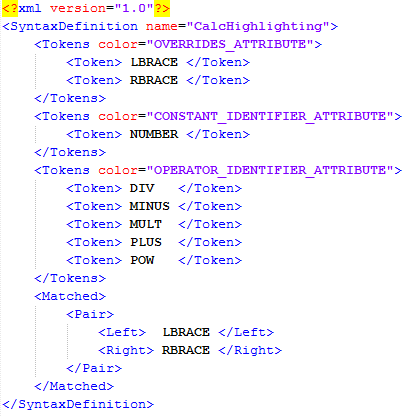
\includegraphics[height=90mm]{Pictures/xmlExample.PNG}
\caption{Пример xml файла.}
\label{xml}
\end{figure}

Поскольку в общем случае неизвестно, какие терминалы будут во входной грамматике и соответственно в какой цвет каждый из них подсвечивать, то автоматизировать привязку к каждому токену определенного цвета невозможно. Поэтому решено на этом этапе также возвращать xml-файл (см. рис. ~\ref{xml}). Он содержит в себе сопоставление “токен -> цвет”. Также в нём поддерживается задание парных символов, что позволяет осуществлять динамическую подсветку (например, для открывающих и закрывающих скобок). 

В генераторе используются цвета, принятые в ReSharper SDK. Для удобства пользователя названия всех доступных цветов указываются в комментариях сгенерированного xml файла. 